%% Based on a TeXnicCenter-Template by Gyorgy SZEIDL.
%%%%%%%%%%%%%%%%%%%%%%%%%%%%%%%%%%%%%%%%%%%%%%%%%%%%%%%%%%%%%

%------------------------------------------------------------
%
\documentclass[letter-size, 11pt]{article}

%%%%%%%%%%%%%%PACKAGES%%%%%%%%%%%%%%%%%%%%%
%%%%%%%%%%%%%%%%%%%%%%%%%%%%%%%%%%%%%%%%%%%
%%%%%%%%%%%%%%%%%%%%%%%%%%%%%%%%%%%%%%%%%%%

%
\usepackage{amsmath}%
\usepackage{amsfonts}%
\usepackage{amssymb}%
\usepackage{dsfont}
%\usepackage{graphicx}
\usepackage[latin1]{inputenc} 
%\usepackage[T1]{fontenc} 
%\usepackage{layout}
%\usepackage{setspace}
\usepackage{tikz}
%\usepackage{algorithm2e}
\usepackage[left=2.8cm,right=2.8cm,top=2cm,bottom=3cm]{geometry}
\usepackage{subcaption}

\usetikzlibrary{decorations}
\usetikzlibrary{decorations.pathmorphing}
\usetikzlibrary{decorations.pathreplacing}
\usetikzlibrary{decorations.shapes}
\usetikzlibrary{decorations.text}
\usetikzlibrary{decorations.markings}
\usetikzlibrary{decorations.fractals}
\usetikzlibrary{decorations.footprints}
%-------------------------------------------
%%%%%%%%%%%%%%THEOREMS%%%%%%%%%%%%%%%%%%%%%
%%%%%%%%%%%%%%%%%%%%%%%%%%%%%%%%%%%%%%%%%%%
%%%%%%%%%%%%%%%%%%%%%%%%%%%%%%%%%%%%%%%%%%%

\newtheorem{theorem}{Theorem}
\newtheorem{definition}{Definition}
\newtheorem{lemma}{Lemma}
\newtheorem{example}{Example}
\newtheorem{corollary}{Corollary}
\newtheorem{problem}{Problem}
\newtheorem{acknowledgement}[theorem]{Acknowledgement}
\newtheorem{axiom}[theorem]{Axiom}
\newtheorem{case}[theorem]{Case}
\newtheorem{claim}[theorem]{Claim}
\newtheorem{conclusion}[theorem]{Conclusion}
\newtheorem{condition}[theorem]{Condition}
\newtheorem{conjecture}[theorem]{Conjecture}

\newtheorem{criterion}[theorem]{Criterion}
\newtheorem{exercise}[theorem]{Exercise}
\newtheorem{notation}[theorem]{Notation}
\newtheorem{proposition}[theorem]{Proposition}
\newtheorem{remark}[theorem]{Remark}
\newtheorem{solution}[theorem]{Solution}
\newtheorem{summary}[theorem]{Summary}
\newenvironment{proof}[1][Proof]{\textbf{#1.} }{\ \rule{0.5em}{0.5em}}

%%%%%%%%%%%%%%COMMANDS%%%%%%%%%%%%%%%%%%%%%
%%%%%%%%%%%%%%%%%%%%%%%%%%%%%%%%%%%%%%%%%%%
%%%%%%%%%%%%%%%%%%%%%%%%%%%%%%%%%%%%%%%%%%%

\newcommand{\kctp}{$k$-CTP}
\newcommand{\set}[1]{\left\{ #1 \right\}}
\newcommand{\card}[1]{\left| #1 \right|}
\newcommand{\ith}[1]{#1^{\mbox{\scriptsize{th}}}}
\newcommand{\stpath}{$(s,t)$-path}
\newcommand{\stpaths}{$(s,t)$-paths}
\newcommand{\omegamin}{\omega_{\mbox{\scriptsize{min}}}}
%Grandes lettres italiques
\newcommand{\mcalp}{\mathcal{P}}
\newcommand{\mcals}{\mathcal{S}}
\newcommand{\mcale}{\mathcal{E}}
\newcommand{\mcalb}{\mathcal{B}}
\newcommand{\mcall}{\mathcal{L}}
\newcommand{\mcalr}{\mathcal{R}}
\newcommand{\mcalt}{\mathcal{T}}


%%%%%%%%%%%%%%DOCUMENT%%%%%%%%%%%%%%%%%%%%%
%%%%%%%%%%%%%%%%%%%%%%%%%%%%%%%%%%%%%%%%%%%
%%%%%%%%%%%%%%%%%%%%%%%%%%%%%%%%%%%%%%%%%%%

\begin{document}

\title{Canadian travellers minimize the traversed distance: definitions, bounds and heuristics}

\maketitle

%\begin{abstract}
%%
%\end{abstract}


%\smallskip
%\begin{center}
%\noindent \textbf{Keywords.} blabla. 
%\end{center}
%\smallskip


\section{Introduction}

The \textit{Canadian Traveller Problem} (CTP) was introduced by Papadimitriou and Yannakakis~\cite{PaYa91}. This is a generalization of the \textit{Shortest Path Problem}. Given an undirected weighted graph $G=(V,E,\omega)$ and two nodes $s,t \in V$, the objective is to design a strategy in order to make a traveller walk from $s$ to $t$ through the graph $G$, knowing that some edges can be blocked. The traveller ignores which edges are blocked when he begins and discover them when he visits an adjacent node. The $k$-\textit{Canadian Traveller Problem} (\kctp) is the parameterized variant of CTP where we specify an upper bound for the total number of blocked edges. Both CTP and \kctp ~are PSPACE-complete~\cite{BaSc91,PaYa91}.

\paragraph{State-of-the-art:}Several strategies have been designed and studied through the competitive analysis, which is a way to assess the quality of an online algorithm. A first class of strategies to be considered are deterministic. Westphal proved that there is no deterministic algorithm that can achieve a better competitive ratio than $2k+1$ where $k$ is an upper bound of the number of blockages and that this ratio is achieved by \textsc{reposition} algorithm~\cite{We08}. However, in practice (for example in the case of an urban network), returning to node $s$ everytime the traveller is blocked does not seem to be an efficient strategy. This is why Xu et al. introduced the \textsc{greedy} algorithm for the CTP which achieves a $2^{k+1}-1$ ratio~\cite{XuHuSuZh09}. For grids, they showed that the \textsc{greedy} strategy achieves a $\mathcal{O}\left(1\right)$ ratio, independent of $k$, under realistic hypotheses. Both \textsc{greedy} and \textsc{reposition} strategies are executed in polynomial time.

A second class of strategies are randomized. We evaluate these strategies by supposing that an oblivious adversary is setting the blocked edges. Westphal proved that there is no randomized algorithm that can achieve a ratio lower than $k+1$~\cite{We08}. Recently, two randomized algorithms have been proposed. Demaine et al. designed a strategy for arbitrary graphs with a ratio $\left(1+\frac{\sqrt{2}}{2}\right)k+1$. This is executed in time $\mathcal{O}\left(k\mu^2\card{E}^2\right)$ where $\mu$ is an parameter that can potentially be exponential~\cite{DeHuLiSa14}. However, for a rather large class of graph (graphs with a reasonable number of groups of path, where a group of path is a set of paths which have the same length), this strategy offers better results than deterministic methods and is executed in polynomial time. Furthermore, Bender et al. studied the specific case of node-disjoint-paths graphs and proposed a strategy of ratio $\left(k+1\right)$ and with a polynomial running time for this kind of graphs~\cite{BeWe15}. Their method consists in a randomized \textsc{reposition}: we assign a probability $p_i$ to each path $P_i$ and execute a draw: the traveller crosses the path and, if he is blocked, returns to $s$ and restarts the process.

% \paragraph{Contributions:} The main objective of this study is to design a randomized strategy which has a $(K+1)$-competitive ratio for graphs $G$. Here is a list of our contributions:
% \begin{itemize}
% \item We introduce the \knctp ~which the two-parameters variant of CTP where $K$ is the upper bounded on the number of blocked edges and $n$ is the exact number of simple \stpaths.
% \item We prove that the competitive ratio of the randomized reposition strategy on $K$-CTP, noted $\arb$, is at least $2k+1$ for any kind of graphs. It implies that this method is specific for a certain class of graphs, containing at least node-disjoint paths instances.
% \item We propose an optimal randomized strategy to treat graphs which fulfils the following condition: there is a $\left(K+1\right)$-partition $\mcalp_1 \cup \ldots \cup \mcalp_{K+1}$ of the set of simple \stpaths ~such that, for any path $P_i \in \mcalp_i$ ,$P_j \in \mcalp_j$, $j\neq i$, $P_i$ and $P_j$ are node-disjoint. Its competitive ratio is $K+1$.
% \item We build a randomized strategy called the Canadian Traveller Random Search (CTRS) for graphs such that simple \stpaths ~have the same cost. We note it $\ars$. The competitive ratio is $K+1$. This randomized strategy is optimal for this kind of instances.
% \end{itemize}

\section{Preliminaries}

\subsection{Notations and definitions with a single traveller} 
The traveller traverses an undirected weighted graph $G=\left(V,E,\omega\right)$, $n = \card{V}$ and $m = \card{E}$. He starts his walk at source $s \in V$. His objective is to reach target $t\in V$ with a minimum cost (also called distance), which is the sum of the weights of edges traversed. Set $E_*$ contains blocked edges, which means that when the traveller reaches an endpoint of one of these edges, he discovers that he cannot pass through it. A pair $\left(G,E_*\right)$ is called a \textit{road map}. From now on, we suppose that any road map $\left(G,E_*\right)$ is feasible, {\em i.e.} $s$ and $t$ are always connected in graph $G\backslash E_*$.

We remind the definition of the competitive ratio introduced in \cite{BoEl98}. Let $\omega_A\left(G,E_*\right)$ be the distance traversed by the traveller guided by a given strategy $A$ on graph $G$ from source $s$ to target $t$ with blocked edges $E_*$. The shortest \stpath ~in $G\backslash E_*$ is called the \textit{optimal offline path} of map $\left(G,E_*\right)$ and its cost, noted $\omegamin\left(G,E_*\right)$, is the optimal offline cost of map $\left(G,E_*\right)$. Strategy $A$ is $c_A$-competitive if, for any road map $\left(G,E_*\right)$:

\[
\omega_A\left(G,E_*\right) \leq c_A\omegamin\left(G,E_*\right) + \eta,
\]
%\label{eq:deter-comp}
where $\eta$ is constant. For randomized strategies, it becomes:

\[
\mathbb{E}\left[\omega_A\left(G,E_*\right)\right] \leq c_A\omegamin\left(G,E_*\right) + \eta.
\]

\subsection{Notations and definitions with $L$ travellers}

The $L$ travelers traverses the same undirected weighted graph $G=\left(V,E,\omega\right)$, $n = \card{V}$ and $m = \card{E}$. They all start their walk at source $s \in V$. Their objective is to reach target $t\in V$ with a minimum cost (also called distance), which is the sum of the weights of edges traversed. We call $d_i$ the distance travelled by the $\ith{i}$ traveler. We consider that the $L$ travelers can communicate with each other. Set $E_*$ contains blocked edges, which means that when a traveller reaches an endpoint of one of these edges, he discovers that he cannot pass through it and communicate this information to the other travelers. A pair $\left(G,E_*\right)$ is called a \textit{road map}. From now on, we suppose that any road map $\left(G,E_*\right)$ is feasible, {\em i.e.} $s$ and $t$ are always connected in graph $G\backslash E_*$.

We consider the following timeline which brings forth three times we will need to study this problem.
\begin{center}
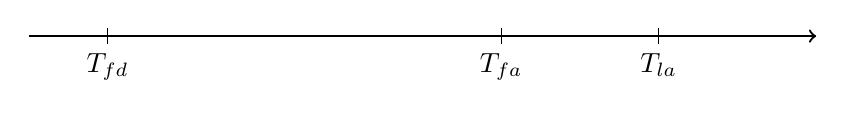
\begin{tikzpicture}
\draw [->] [thick] (0,0)--(10,0);
\draw (1,-.1) node[below]{$T_{fd}$}--(1,.1);
\draw (6,-.1) node[below]{$T_{fa}$}--(6,.1);
\draw (8,-.1) node[below]{$T_{la}$}--(8,.1);
\end{tikzpicture}
\end{center}
\[
T_{fd} \mbox{\ : time of the first departure}
\]
\[
T_{fa} \mbox{\ : time of the first arrived}
\]
\[
T_{la} \mbox{\ : time of the last arrived}
\]

We want to study the minimization of the distances traversed by all the travelers from the departure point $s$ and the arrival point $t$. We consider $d_i$ the distance traversed by the $\ith{i}$ traveler. We have two main problems to consider, we will try to minimize the distances traversed by all travelers:
\begin{description}
\item[$\bullet$] Before the first arrived :
\[ 
\sum_{i=1}^{L} d_{i} \mbox{\qquad between } T_{fd} \mbox{\ and } T_{fa}
\]
\item[$\bullet$] After the last arrived :
\[ 
\sum_{i=1}^{L} d_{i} \mbox{\qquad between } T_{fd} \mbox{\ and } T_{la}
\]
\end{description}



\section{Bounds of competitiveness: deterministic algorithms}

We will study this problem with three different types of communication. We will note $P_0$ the proposition when we don't have any communication, $P_1$ when we have partial communication and $P_2$ for complete communication.

\subsection{Complete communication}

We consider the following deterministic and online algorithm for $K$ blocked edges and $L$ travellers with complete communication: we launch the travellers one at a time. If the traveller meets a blocked edge, it has to stay there and we launch another traveller who will have to take the second shortest path possible. Once again when this one meets a blocked edge, it stays there and another is launched. Let's call this strategy the $\textsc{abandonment}$ strategy.


\begin{lemma} The cost of the abandonment strategy on the Westphal graph is $2(K+1) - \min(K+1,L)$ between $T_{fd}$ and $T_{fa}$ and $2K+L$ between $T_{fd}$ and $T_{la}$.
\end{lemma}


\begin{proof}We consider the following Westphal graph, where all the ways from the departure point to the arrival point have the same cost $1+\varepsilon$. We are searching the cost for the worst case scenario: the only unblocked route is the one we choose last $(s,v_{K+1},t)$.

\begin{center}
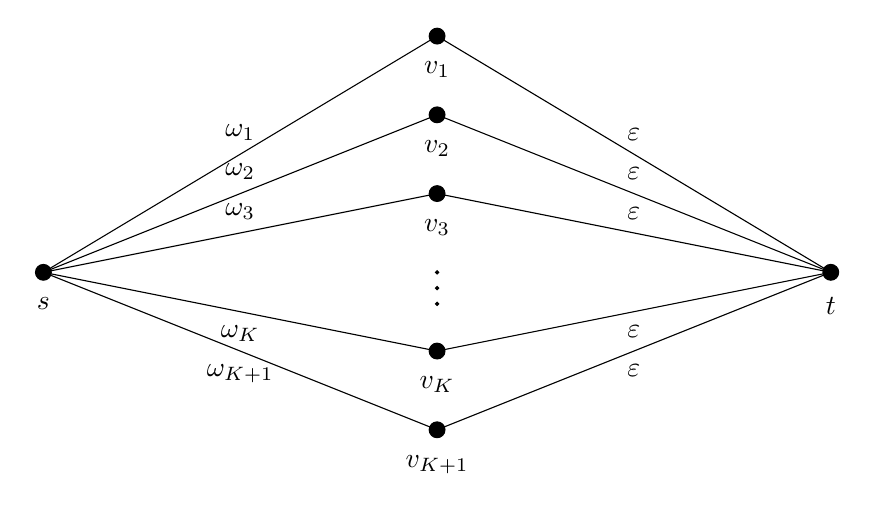
\begin{tikzpicture}
\foreach \Point/\PointLabel in {(0,2)/s, (10,2)/t, (5,0)/v_{K+1}, (5,1)/v_{K}, (5,3)/v_3, (5,4)/v_2, (5,5)/v_1}
    \draw[fill=black] \Point circle (0.1) node[below = 0.2cm] {$\PointLabel$};
\foreach \Point in {(5,1.6), (5,1.8), (5,2)}
    \draw[fill = black] \Point circle (0.02);
\foreach \Point in {(5,0), (5,1), (5,3), (5,4), (5,5)}
    \draw \Point -- (0,2);
\foreach \Point in {(5,0), (5,1), (5,3), (5,4), (5,5)}
    \draw \Point -- (10,2);
    \foreach \Point/\PointLabel/\Position in {(2.5,1)/\omega_{K+1}/below, (2.5,1.5)/\omega_{K}/below, (2.5,2.5)/\omega_3/above, (2.5,3)/\omega_2/above, (2.5,3.5)/\omega_1/above,(7.5,1)/\varepsilon/below, (7.5,1.5)/\varepsilon/below, (7.5,2.5)/\varepsilon/above, (7.5,3)/\varepsilon/above, (7.5,3.5)/\varepsilon/above}
    \draw \Point node[\Position = 0.05cm] {$\PointLabel$};
\end{tikzpicture}
\end{center}

We consider that $w_1 = w_2 = ... = w_{K+1} = 1$, that $\varepsilon$ is very small, that for $1\leq i \leq K$, $(v_i,t)$ is blocked and that $t_{i+1}$ is a time after the $i^{th}$ movement.

We have in fact 4 problems to consider: for each of the 2 main problems (between $T_{fd}$ and $T_{fa}$ and between $T_{fd}$ and $ T_{la}$) we have two secondary problems, when $K<L$ and ${K \geq L}$.

\begin{description}
\item[$\bullet$] Case 1: between $T_{fd}$ and $T_{fa}$ and $K<L$

At the time $t_1$, we send a first traveler through the edge $(s,v_1)$, who discovers that the edge $(v_1,t)$ is blocked and communicates it to the other travelers.

Then we send at the times $t_i$ with $1 < i \leq K$ a traveler through the edge $(s,v_i)$ and discovers that the edge $(v_i,t)$ is blocked and communicates it to the other travelers.

At the time $t_{K+1}$, we send a traveler through the edges $(s,v_{K+1})$ and then reaches the destination by the edge $(v_{K+1},t)$. 

Therefore we have: 
\[
\sum_{i=1}^{K} \omega_{i} + \omega_{K+1} + \varepsilon = \sum_{i=1}^{K} 1 + 1 + \varepsilon = K + 1 + \varepsilon.
\]

\item[$\bullet$] Case 2: between $T_{fd}$ and $T_{la}$ and $K<L$

We redo the three first steps of the 1st case and at $ T_{pa} $ the first traveler communicate the unblocked route to the target and therefore that the edge $(v_{K+1},t)$ is not blocked.

At the time $t_{K+2}$ the K travelers blocked on the nodes $v_{1} ... v_K $ come back to the point s and then take the unblocked route $(s,v_{K+1},t)$. The $L-K-1$ travelers who have not left, take the unblocked route $(s,v_{K+1},t)$.

Each traveler at the point $v_i$ will then arrive at the destination with a cost of $w_i + w_{K+1} + \varepsilon$. And each traveler still at the departure point will arrive at destination with a cost of $w_{K+1} + \varepsilon$.

Therefore, we have:
\begin{eqnarray}
\sum_{i=1}^{K} \omega_{i} &+& \omega_{K+1} + \varepsilon + \sum_{i=1}^{K}(\omega_{i} + \omega_{K+1} + \varepsilon) + (L - K) ( \omega_{K+1} + \varepsilon ) \nonumber \\
&=& 2\sum_{i=1}^{K} \omega_{i} + L(\omega_{K+1} + \varepsilon ) = 2\sum_{i=1}^{K} 1+ L(1 + \varepsilon ) \nonumber \\
&=& 2K+ L(1 + \varepsilon ). \nonumber
\end{eqnarray}


\item[$\bullet$] Case 3: between $T_{fd}$ and $T_{fa}$ and $K \geq L$

At the time $t_1$, we send a first traveler through the edge $(s,v_1)$, who discovers that the edge $(v_1,t)$ is blocked and communicates it to the other travelers.

Then we send at the times $t_i$ with $1 < i \leq L$ a traveler through the edge $(s,v_i)$ and discovers that the edge $(v_i,t)$ is blocked and communicates it to the other travelers.

At the time $t_{L+1}$, we send the traveler which is at the point $v_l$ through the edges $(v_{L},s)$ and then $(s,v_{L+1})$. He discovers that the edge $(v_{L+1},t)$ is blocked and communicates it to the other travelers.

Then we send at the times $t_i$ with $L+1 < i \leq K$ a traveler through the route $(v_{i-1},s,v_i)$ and discovers that the edge $(v_i,t)$ is blocked and communicates it to the other travelers.

At the time $t_{K+1}$, we send a traveler through the route $(v_K,s,v_{K+1})$ and then reaches the destination by the edge $(v_{K+1},t)$. 

Therefore we have: 

\begin{eqnarray}
\sum_{i=1}^{L} \omega_{i} &+& \sum_{i=L+1}^{K}(\omega_{i-1} + \omega_{i} ) + \omega_{K} + \omega_{K+1} + \varepsilon  \nonumber\\
&=&\sum_{i=1}^{L} 1 + \sum_{i=1}^{K-L}2 + 1 + 1 + \varepsilon\nonumber \\
&=& L + 2(K - L) + 2 + \varepsilon \nonumber\\
&=& 2(K + 1 ) - L + \varepsilon.\nonumber
\end{eqnarray}

\item[$\bullet$] Case 4: between $T_{fd}$ and $T_{la}$ and $K \geq L$

We redo the five first steps of the third case and at $ T_{pa}$ the first traveler will communicate the unblocked route to the target and therefore that the edge $(v_{K+1},t)$ is not blocked.

At the time $t_{K+2}$ the L-1 travelers blocked on the nodes $v_{1} ... v_{L-1} $ come back to the point s and then take the unblocked route $(s,v_{K+1},t)$.

Each traveler at the point $v_i$ will then arrive at the destination with a cost of $w_i + w_{K+1} + \varepsilon$. 

Therefore we have:

\begin{eqnarray}
2(K + 1) & - & L + \varepsilon + \sum_{i=1}^{L-1}(\omega_{i} + \omega_{K+1} + \varepsilon ) \nonumber\\
& = & 2K + L(1+\varepsilon).\nonumber
\end{eqnarray}


\end{description}
\end{proof}

Therefore we have the following costs for the Westphal graph:

\begin{center}
\begin{tabular}{|c|c|c|}
\hline
 & between $T_{fd}$ and $T_{fa}$  & between $T_{fd}$ and $ T_{la}$ \\ 
\hline
 ${K<L}$  & ${K + 1}$ & ${ 2K + L}$   \\ 
\hline
 ${K \geq L}$  & ${2(K+1) - L}$ & ${2K + L}$   \\ 
\hline
\end{tabular}
\end{center}

\begin{lemma} The abandonment strategy has the optimal cost on the Westphal graph.
\end{lemma}

\begin{proof} This Lemma is proved using recurrence.  

\paragraph{Recurrence hypothesis:} For K (blocked edges), for all $L$ the optimal cost is : $K + 1$ if $L > K$ and $2K - L + 1$ if $L < K$.

\paragraph{Initialization:} Let us take the example of $L = 1$ traveler. As shown in the existing literature we already have the cost equal to $K + 1$.

\paragraph{Recurrence:} We know that there is a natural integer n number of travellers for which the cost is: if $n > K$, the cost is $K + 1$, and if $n < K$, the cost is $2K - L + 1$. Let's prove it for $n + 1$. 
If $n + 1 < K$, since we are in the worst case scenario, the $n$ travellers have to discover the $K$ blocked edges before reaching the end. To do so, the cost is at least of $K$. Then $1$ is added to reach the end. However, our strategy has a cost of $K + 1$ also, therefore once again, for$ n + 1 < K$, the optimal cost is $K + 1$. 

Now if $n + 1 > K$, we launch the first traveler. He discovers one blocked edge and stays there. We are now facing a problem of $n$ travllers facing $K-1$ blockage. By recurrence hypothesis we know that for that case the cost is $2(K-1) - n + 1$ because $n > K - 1$. To that cost we add the cost of discovering the first blocked edge. We have $2(K + 1) - n + 2$ which is equal to $2K - (n + 1) - 1$. This shows the second part of the recurrence.

We can therefore conclude that the optimal cost for the Westphal graph is : $K + 1$ if $L > K$ and $2K - L + 1$ if $L < K$. This is the cost of the abandonment strategy. 
\end{proof}

\begin{lemma} The competitive ratios found in the Lemma 3.1.1 are the minimum we can have for any graph. Therefore the best competitive ratio for the abandonment algorithm is $2(K+1) - min(K+1,L)$ between $T_{fd}$ and $T_{fa}$ and $2K+L$ between $T_{fd}$ and $T_{la}$.
\end{lemma}

\begin{proof} We consider the same graph as in the proof of the Lemma 3.1, but this time we consider that we have $w_1 < w_2 < ... < w_{K+1}$. We still consider that $\varepsilon$ is very small, that for $1\leq i \leq K$, $(v_i,t)$ is blocked and that $t_{i+1}$ is a time after the $i^{th}$ movement. We are still searching for the cost of the worst case scenario: the only unblocked route is the one we choose last, in this case the one with the biggest cost $(s,v_{K+1},t)$.


We still have the same 4 problems to study as in the proof of the Lemma 3.1.1, for each case, we follow the same procedure as before.

The true optimum route in each case will be the last one taken with a cost of $\omega_{K+1} + \varepsilon$.

\begin{description}
\item[$\bullet$] Case 1: between $T_{fd}$ and $T_{fa}$ and $K<L$

We have: 
\begin{eqnarray}
\frac {\sum_{i=1}^{K} \omega_{i} + \omega_{K+1} + \varepsilon} {\omega_{K+1} + \varepsilon} &\leq& \frac {\sum_{i=1}{K+1} \omega_{K+1} +} {\omega_{K+1}} + o(1)  \nonumber \\
\leq \frac {(K+1)\omega_{K+1} } {\omega_{K+1}} + o(1) &\leq& K+1 + o(1).\nonumber
\end{eqnarray}

\item[$\bullet$] Case 2: between $T_{fd}$ and $T_{la}$ and $K<L$

We have:
\[
\frac {\sum_{i=1}^{K} \omega_{i} +  \omega_{K+1} + \varepsilon + \sum_{i=1}^{K}(\omega_{i} + \omega_{K+1} + \varepsilon) + (L - K) ( \omega_{K+1} + \varepsilon )}{\omega_{K+1} + \varepsilon}
\]
\begin{eqnarray}
&\leq& \frac {2\sum_{i=1}^{K} \omega_{K+1} + L\omega_{K+1}}{\omega_{K+1}} + o(1) \leq \frac {2(K+L)\omega_{K+1}}{\omega_{K+1}} + o(1) \nonumber\\
 &\leq& 2K+ L + o(1).\nonumber
\end{eqnarray}

\item[$\bullet$] Case 3: between $T_{fd}$ and $T_{fa}$ and $K \geq L$

We have: 

\begin{eqnarray}
\frac {\sum_{i=1}^{L} \omega_{i} + \sum_{i=L+1}^{K}(\omega_{i-1} + \omega_{i} ) + \omega_{K} + \omega_{K+1} + \varepsilon} {\omega_{K+1} + \varepsilon} 
&\leq& \frac {\sum_{i=1}^{L} \omega_{K+1} + \sum_{i=1}^{K-L}2\omega_{K+1} + 2\omega_{K+1}}{\omega_{K+1}} + o(1) \nonumber\\
\leq \frac {(L + 2(K - L) + 2)\omega_{K+1}}{\omega_{K+1}} + o(1)
&\leq& 2(K + 1 ) - L + o(1).\nonumber
\end{eqnarray}

\item[$\bullet$] Case 4: between $T_{fd}$ and $T_{la}$ and $K \geq L$

We have:

\[
\frac {\sum_{i=1}^{L} \omega_{i} + \sum_{i=L+1}^{K}(\omega_{i-1} + \omega_{i} ) + \omega_{K} + \omega_{K+1} + \varepsilon + \sum_{i=1}^{L-1}(\omega_{i} + \omega_{K+1} + \varepsilon } {\omega_{K+1} + \varepsilon} 
\]
\begin{eqnarray}
&\leq& \frac {\sum_{i=1}^{L} \omega_{K+1} + \sum_{i=1}^{K-L}2\omega_{K+1} + 2\omega_{K+1} + \sum_{i=1}^{L-1}(\omega_{K+1} + \omega_{K+1}} {\omega_{K+1}} + o(1) \nonumber\\
&\leq& \frac {(L + 2(K - L) + 2 + 2(L-1)\omega_{K+1}}{\omega_{K+1}} + o(1)
 \leq 2K + L + o(1).\nonumber
\end{eqnarray}

\end{description}
\end{proof}

Therefore we have the following competitive ratio for any graph:

\begin{center}
\begin{tabular}{|c|c|c|}
\hline
 & between $T_{fd}$ and $T_{fa}$  & between $T_{fd}$ and $ T_{la}$ \\ 
\hline
 ${K<L}$  & ${K + 1}$ & ${ 2K + L}$   \\ 
\hline
 ${K \geq L}$  & ${2(K+1) - L}$ & ${2K + L}$   \\ 
\hline
\end{tabular}
\end{center}

\subsection{No communication}
We now consider the same following deterministic and online algorithm for K blocked edges and L travellers with no communication: they don't even know that they are a part of a fleet, so they will all leave at the first moment and will all arrive at the same time at the end point. We will call this strategy the multiple single traveler strategy.

\begin{lemma} The cost of the multiple single traveler strategy on the Westphal graph is $(2K+1)L$ between $T_{fd}$ and $T_{fa}$ and between $T_{fd}$ and $T_{la}$.
\end{lemma}

\begin{proof} None of the L travelers know that they are a fleet. All of them will depart at the first time. We are in the worst case scenario, so all of them will go through all the blocked paths before finding the opened one. They will all be independent and act as a single traveler. They will all arrive at the destination at the same time. Therefore no matter if we take into account the distance between $T_{fd}$ and $T_{fa}$ or between $T_{fd}$ and $T_{la}$, we will have a cost of $(2K+1)$ for each traveler, meaning $(2K+1)L$ total.
\end{proof}

\begin{lemma}The multiple single traveler strategy has the optimal cost on the Westphal graph.
\end{lemma}

\begin{proof} All of the travelers aren't communicating, therefore they are independent. We are in the worst case scenario, so each traveler will be as a single traveler and have a cost of $(2K+1)$ as seen in the existence literature. So we have a total cost of $(2K+1)L$.
\end{proof}

\begin {lemma} The competitive ratios found in the Lemma 3.2.1 are the minimum we can have for any graph. Therefore the best competitive ratio for the multiple single traveler algorithm is $(2K+1)L)$ between $T_{fd}$ and $T_{fa}$ and between $T_{fd}$ and $T_{la}$.
\end{lemma}

\begin {proof} We consider the same graph as in the proof of the Lemma 3.2.1, but this time we consider that we have $w_1 < w_2 < ... < w_{K+1}$. We still consider that $\varepsilon$ is very small, that for $1\leq i \leq K$, $(v_i,t)$ is blocked. We are still searching for the cost of the worst case scenario: the only unblocked route is the one we choose last, in this case the one with the biggest cost $(s,v_{K+1},t)$.

The optimum route which is the only unblocked route in each case will be the last one taken with a cost of $\omega_{K+1} + \varepsilon$.

In both cases, we will have:
\begin{eqnarray}
\frac {L(\sum_{i=1}^{K} 2*\omega_{i} + \omega_{K+1} + \varepsilon)} {\omega_{K+1} + \varepsilon} 
&\leq& \frac {L(\sum_{i=1}^{K} 2*\omega_{K+1} + \omega_{K+1})} {\omega_{K+1}} + o(1) \nonumber\\
\leq \frac {L(2K+1)\omega_{K+1} } {\omega_{K+1}} + o(1)
&\leq& L(2K+1) + o(1).\nonumber
\end{eqnarray}

For any graph, the best competitive ratio for the multiple single travaler strategy is $L(2K+1)$ for both problems: between $T_{fd}$ and $T_{fa}$ and between $T_{fd}$ and $T_{la}$.
\end{proof}

\subsection{Partial communication}
We now consider the same following deterministic and online algorithm for $K$ blocked edges and $L$ travelers with partial communication: the travelers can communicate at the beginning and decide what each traveler will do, they don't talk later on. We will have a rolling strategy where the first traveler takes the first route, the second one will wait a time a bit bigger than it would have taken the first one to arrive at destination if the first path was unblocked, and will take the second path and so on. In the cases where $K>L$ the last traveler will continue to take each following path when we are in the fist arrival problem. For the last arrival problem, we will minimize the worst case scenario by eliminating some paths for travelers as they will take different paths at the beginning and take the following one afterwards. Therefore they will not all be travelling all paths.

\begin{lemma} The cost of the rolling travelers strategy on the Westphal graph is:

\begin{center}
\begin{tabular}{|c|c|c|}
\hline
 & between $T_{fd}$ and $T_{fa}$  & between $T_{fd}$ and $ T_{la}$ \\ 
\hline
 ${K<L}$  & ${K + 1}$ & ${2K + L - \lfloor \frac{L}{K+1} \rfloor(K+1)(K+2) - (L-\lfloor \frac{L}{K+1} \rfloor)(L-\lfloor \frac{L}{K+1} \rfloor + 1)}$   \\ 
\hline
 ${K \geq L}$  & ${2(K+1) - L}$ & ${ 2K - L^2}$   \\ 
\hline
\end{tabular}
\end{center}
\end{lemma}

\begin{proof} We consider the same Westphal graph as in the proof of the Lemma 3.1.1 and the same 4 problems. We consider that the times $t_i$ is i times the time needed to go from s to t with an unblocked path (in this case time needed to travel $1 + \varepsilon$). 

\begin{description}
\item[$\bullet$] Case 1: between $T_{fd}$ and $T_{fa}$ and $K<L$

At the time $t_1$, we send a first traveler through the edge $(s,v_1)$, who discovers that the edge $(v_1,t)$ is blocked and stays there.

Then we send at the times $t_i$ with $1 < i \leq K$ a traveler through the edge $(s,v_i)$ and discovers that the edge $(v_i,t)$ is blocked and stays there.

At the time $t_{K+1}$, we send a traveler through the edges $(s,v_{K+1})$ and then reaches the destination by the edge $(v_{K+1},t)$. 

Therefore we have: 
\[
\sum_{i=1}^{K} \omega_{i} + \omega_{K+1} + \varepsilon = \sum_{i=1}^{K} 1 + 1 + \varepsilon = K + 1 + \varepsilon.
\]

\item[$\bullet$] Case 2: between $T_{fd}$ and $T_{fa}$ and $K \geq L$

At the time $t_1$, we send a first traveler through the edge $(s,v_1)$, who discovers that the edge $(v_1,t)$ is blocked ans stays there.

Then we send at the times $t_i$ with $1 < i \leq L$ a traveler through the edge $(s,v_i)$ and discovers that the edge $(v_i,t)$ is blocked and stays there.

At the time $t_{L+1}$, we send the traveler which is at the point $v_L$ through the edges $(v_{L},s)$ and then $(s,v_{L+1})$. He discovers that the edge $(v_{L+1},t)$ is blocked and continues to the next path.

Then we send at the times $t_i$ with $L+1 < i \leq K$ the same last traveler through the route $(v_{i-1},s,v_i)$ and discovers that the edge $(v_i,t)$ is blocked and continues.

At the time $t_{K+1}$, we send the last traveler through the route $(v_K,s,v_{K+1})$ and then reaches the destination by the edge $(v_{K+1},t)$. 

Therefore we have: 

\begin{eqnarray}
\sum_{i=1}^{L} \omega_{i} + \sum_{i=L+1}^{K}(\omega_{i-1} + \omega_{i} ) + \omega_{K} + \omega_{K+1} + \varepsilon
&=&\sum_{i=1}^{L} 1 + \sum_{i=1}^{K-L}2 + 1 + 1 + \varepsilon \nonumber\\
= L + 2(K - L) + 2 + \varepsilon
&=& 2(K + 1 ) - L + \varepsilon.\nonumber
\end{eqnarray}

\item[$\bullet$] Case 3: between $T_{fd}$ and $T_{la}$ and $K \geq L$

At the time $t_1$, we send the $i^{th}$ traveler through the edges $(s,v_i)$ for $1 \leq i \leq L$ they all discover that the edge $(v_i,t)$ is blocked.

For each time $t_j$, with $1 \leq j \leq L-K$ we will send all the travelers through the following path. The $i^{th}$ traveler through the edges $(s,v_{i+j-1})$ for $1 \leq i \leq L$, all discover that the edge $(v_{i+1},t)$ is blocked.

For each following time $t_j$, with $L-K < j \leq L$ we will send all the travelers through the following path. The $i^{th}$ traveler through the edges $(s,v_{i+j-1})$ for $1 \leq i \leq L-K-j$, all discover that the edge $(v_{i+1},t)$ is blocked except the last one who arrives at destination and stays there.

The first traveler will then have a cost of $2K+1$, the second of $2K$. For $1 \leq i \leq L$, the $i^{th}$ traveler will have a cost of $2(K-i)+1$

Therefore we have:

\begin{eqnarray}
\sum_{i=1}^{L}(2(K-i)+1)
&=& 2KL + L - 2\sum_{i=1}^{L}i
= L(2K+1) - 2\frac{L(L+1)}{2} \nonumber \\
&=& L(2K + 1-(L+1))
= L(2K - L).\nonumber
\end{eqnarray}

\item[$\bullet$] Case 4: between $T_{fd}$ and $T_{la}$ and $K<L$

We redo the same pattern as in the 3rd case, but there will be more than one traveler on the same road. The $i^{th}$ traveler will take the $i\bmod{(K+1)}^{th}$ path.

The first traveler will then have a cost of $2K+1$, the second of $2K$. For $1 \leq i \leq L$, the $i^{th}$ traveler will have a cost of $2(K-i\bmod{(K+1)})+1$

Therefore we have:

\begin{eqnarray}
\phi(K,L) &=& \sum_{i=1}^{L}(2(K-(i-1)\bmod{(K+1)})+1) \nonumber \\
&=& L(2K+1) - 2\sum_{i=0}^{L-1}i\bmod{(K+1)} \nonumber \\
&=& L(2K + 1) - 2\left(\left\lfloor \frac{L-1}{K+1} \right\rfloor \sum_{i=0}^{K}i + \sum_{i=0}^{(L-1)\bmod(K+1)}i\right) \nonumber \\
&=& L(2K + 1) - 2\left(\left\lfloor \frac{L-1}{K+1} \right\rfloor\frac{K(K+1)}{2} + \frac{\left((L-1)\bmod(K+1)\right)\left((L-1)\bmod(K+1) + 1\right)}{2}\right)\nonumber \\
&=& L(2K + 1) - \left\lfloor \frac{L-1}{K+1} \right\rfloor K(K+1)- \left((L-1)\bmod(K+1)\right)\left((L-1)\bmod(K+1) + 1\right).\nonumber
\end{eqnarray}

\end{description}
\end{proof}

\subsection{Conclusion for the deterministic approach}

\begin{center}
\begin{tabular}{|c|c|c|c|c|c|}
\hline
 & $P_0$ & \multicolumn{2}{c|}{$P_1$} & \multicolumn{2}{c|}{$P_2$} \\ 
 \hline
 & & $K<L$ & $K\geq L$ & $K<L$ & $K\geq L$\\ 
\hline
 between $T_{fd}$ and $T_{fa}$  & ${2K + 1}$ & ${K+1}$ & ${2(K+1)-L}$ & ${K+1}$ & ${2(K+1)-L}$     \\ 
\hline
between $T_{fd}$ and $ T_{la}$  & ${2K+1}$ & $\phi(K,L)$ & ${ L(2K - L)}$ & ${2K+L}$  & ${2K+L}$ \\ 
\hline
\end{tabular}
\end{center}

In order to have a better view of what $\phi(K,L)$ represents, we propose to the reader to look at the following graphs:

First we set K and make L vary:
%\begin{figure*}
%    \centering
%    \begin{subfigure}[H]{0.475\textwidth}
%            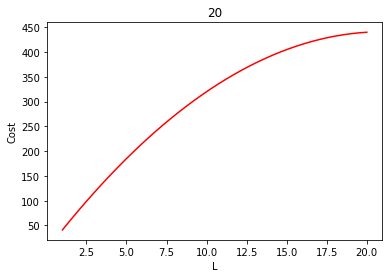
\includegraphics[width=\textwidth]{K20E.png}
%            \caption{$K$ set to 20}
%            \label{a}
%    \end{subfigure}
%    \begin{subfigure}[H]{0.475\textwidth}
%            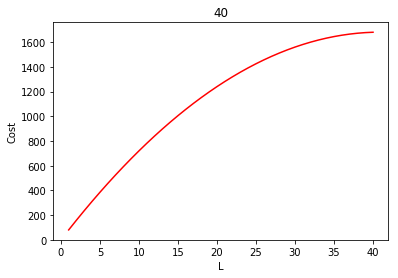
\includegraphics[width=\textwidth]{K40E.png}
%            \caption{$K$ set to 40}
%            \label{b}
%    \end{subfigure}
%
%    \begin{subfigure}[H]{0.475\textwidth}
%            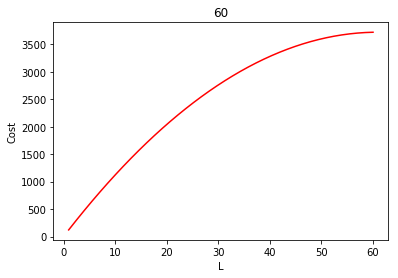
\includegraphics[width=\textwidth]{K60E.png}
%            \caption{$K$ set to 60}
%            \label{c}
%    \end{subfigure}
%    \begin{subfigure}[H]{0.475\textwidth}
%            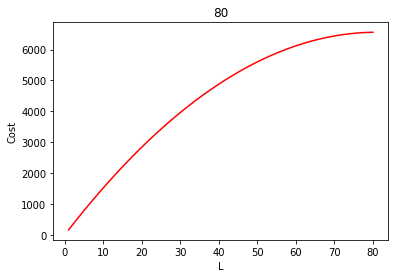
\includegraphics[width=\textwidth]{K80E.png}
%            \caption{$K$ set to 80}
%            \label{d}
%    \end{subfigure}
%    \caption{$K$ set to different values}\label{fig:ABCD}
%\end{figure*}

Then we set $L$ and make $K$ vary:

%\begin{figure*}[h!]
%    \centering
%    \begin{subfigure}[b]{0.475\textwidth}
%            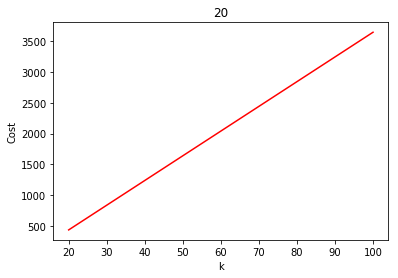
\includegraphics[width=\textwidth]{L20E.png}
%            \caption{$L$ set to 20}
%            \label{a}
%    \end{subfigure}
%    \begin{subfigure}[b]{0.475\textwidth}
%            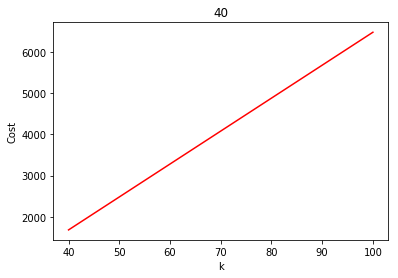
\includegraphics[width=\textwidth]{L40E.png}
%            \caption{$L$ set to 40}
%            \label{b}
%    \end{subfigure}
%
%    \begin{subfigure}[b]{0.475\textwidth}
%            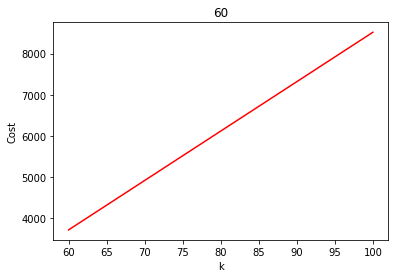
\includegraphics[width=\textwidth]{L60E.png}
%            \caption{$L$ set to 60}
%            \label{c}
%    \end{subfigure}
%    \begin{subfigure}[b]{0.475\textwidth}
%            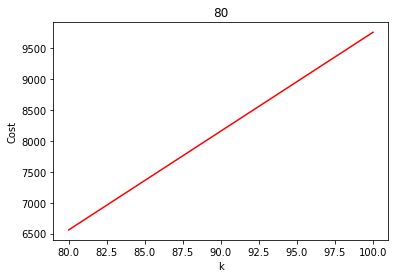
\includegraphics[width=\textwidth]{L80E.png}
%            \caption{$L$ set to 80}
%            \label{d}
%    \end{subfigure}
%    \caption{$L$ set to different values}\label{fig:ABCD}
%\end{figure*}

As one can expect, those curves are rising characteristic curves. Therefore the more travelers, the more blockages, the higher the cost. Nevertheless, one can notice that for a fixed number of blockages, the cost increases less as the number of travelers increase. The cost of getting one more traveler to the destination is then less important.


\section{Bounds of competitiveness: randomized algorithms}
\subsection{Complete communication}
% K blocked edges, L travellers, complete communication
Now we consider the randomized online algorithms for $K$ blocked edges and $L$ travellers with complete communication: we assign a probability $p_i$ to each path $P_i$ and execute a draw: let the travellers crosses the path one by one, if the first traveller is blocked, leave him at the blocked point and let the second traveller to start the process; if all the travellers are blocked, then let the first traveller return to $s$ and restarted the process. 
We can get:

\begin{lemma}
If we have more travellers than blocked edges, there is no randomized online algorithm with competitive ratio less than $\frac{k+2}{2}$.
\label{lemma_moretr}
\end{lemma}

\begin{proof} 
With $K$ smaller than $L$, it is certain that we do not have to let a traveller return to s before we find all the blocked edges. If the algorithm is successful on its $(l+1)^{\text{th}}$ try, only the $(l+1)^{\text{th}}$ try cost ($1+ \eta$) and so the total cost will be:
\[
(l-1)\cdot 1 + (1+\eta) = l+\eta
\]
and the probability will be: 
\[
\frac{1}{l+1}
\]
Hence, its expected cost is at least:
\[
\sum_{l=1}^{k+1}(l+\eta)\cdot \frac{1}{l+1} = \frac{K+2}{2}+\eta
\]
As we know, the expected optimal offline cost is $1 + \eta$, so the competitive ratio is 
\[
\frac{K+2}{2} .
\]
\end{proof}

\begin{lemma}
If we have less travellers than blocked edges $ (K > L )$, there is no randomized online algorithm with competitive ratio less than $
K+2-L+ \frac{L(L-1)}{2(K+1)}$.
\end{lemma}

\begin{proof}
Similar with the proof of Lemma~\ref{lemma_moretr}, if the algorithm is successful on its $(l+1)^{\text{th}}$ try, the probability will be: 
\[
\frac{1}{l+1}
\]
But to calculus the cost, we have to consider two possibilities: 
\\if $l < L$, which means we have find all the blocked edges without letting any traveller to return to $s$, the cost will be 
\[
(l-1)\cdot1 + 1 +\eta = l + \eta;
\]
if $l > L$, it means that we have not find all the blocked edges after letting all the travellers depart $s$,  so we have to let $(l-L)$ travellers return to $s$ and restart the process. In this case, there will be $L$ travellers with cost 1, $(l-L-1)$ travellers with cost 2 and the last traveller with cost $(2+\eta)$. So the total cost will be:
\[
L\cdot 1 + (l-L-1)\cdot2 + 2 +\eta = 2l - L + \eta .
\]
So, its expected cost is at least:
\[
\sum_{l=1}^{L}(l+\eta)\cdot \frac{1}{l+1}  +  \sum_{L+1}^{K+1}(2l-L+\eta)\cdot \frac{1}{l+1}
 =K+2-L+ \frac{L(L-1)}{2(K+1)} + \eta
\]
As we know, the expected optimal off-line cost is $1 + \eta$, so the competitive ratio is 
\[
K+2-L+ \frac{L(L-1)}{2(K+1)}
\]
\end{proof}

If we consider the special case $L=1$ which means only one traveller, the competitive ratio becomes:
\[
K+2-L+ \frac{L(L-1)}{2(K+1)} = K+2-1 = K+1
\]
This result corresponds to the randomized case of Bender et al.~\cite{BeWe15}.

\subsection{No communication}

% K blocked edges, L travellers, complete communication
In the last part, we have discussed randomized online algorithms with total communication, where all the travellers can both send and receive messages. Now we will begin to study randomised cases without communication. 

\begin{lemma}
Considering the distance taken by all travellers after the last arrived (distance between $T_{fd} \mbox{\ and } T_{la}$), there is no randomized online algorithm with competitive ratio less than $ L(K+1)$.
\end{lemma}

\begin{proof} 
According to the result of Bender et al.~\cite{BeWe15}, in randomized case, the competitive ratio for only one traveller is $K+1$. When there is no communication between the travellers, all the travellers make choices independently. In this case, all the $L$ travellers have to reach the target, so the obviously the result becomes $L$ times $K+1$.
\end{proof}

\begin{lemma}
Considering the distance taken by all travellers before the first arrived (distance between $T_{fd} \mbox{\ and } T_{fa}$), there is no randomized online algorithm with competitive ratio less than:
\begin{equation}
\sum_{l=1}^{K+1}\frac{(K-t+2)^{L} - (K-t+1)^{L}}{(K+1)^{L}}\cdot (\frac{2l-2}{L}+1)
\label{cr_rand}
\end{equation}
\end{lemma}

In this case, we have made an assumption which is different from the cases with complete communication: in the beginning, instead of setting off one by one, all the travellers set off together, which is more meaningful in the real world. So when the first travellers reached the target, the travellers, who had set off together with these lucky travellers but were blocked, are on the way back to the source $s$.

\begin{proof} 
\\The probability that the algorithm is successful on its $1^{\text{th}}$ try is: $1-(\frac{K}{K+1})^{L}$;
\\The probability that the algorithm is successful on its $2^{\text{th}}$ try is: $(\frac{K}{K+1})^{L} \cdot [1-(\frac{K-1}{K})^{L}]$;
\\The probability that the algorithm is successful on its $l^{\text{th}}$ try is: 
\[
\ (\frac{K}{K+1})^{L} \cdot  (\frac{K-1}{K})^{L}\cdots  (\frac{K-l+2}{K-l+3})^{L}\cdot [1-(\frac{K-l+1}{K-l+2})^{L}] = \frac{(K-t+2)^{L} - (K-t+1)^{L}}{(K+1)^{L}}
\]
And according to the assumption, the cost will be: $(1+\eta)\cdot L + 2(l-1) $, so the total expected cost is:
\[
\sum_{l=1}^{K+1}\frac{(K-t+2)^{L} - (K-t+1)^{L}}{(K+1)^{L}}\cdot ((1+\eta)\cdot L + 2(l-1) )
\]
As the expected optimal off-line cost is $L(1 + \eta)$, so we can find the result (\ref{cr_rand}).
\end{proof}

\subsection{Conclusion for randomized approaches} 

\begin{center}
\begin{tabular}{|c|c|c|c|}
\hline
 & $P_0$ & \multicolumn{2}{c|}{$P_2$} \\ 
 \hline
 & & $K<L$ & $K\geq L$ \\ 
\hline
 between $T_{fd}$ and $T_{fa}$  & $\sum_{l=1}^{K+1}\frac{(K-t+2)^{L} - (K-t+1)^{L}}{(K+1)^{L}}\cdot (\frac{2l-2}{L}+1)$ & $\frac{K+2}{2}$ & $K+2-L+\frac{L(L-1)}{2(K+1)}$     \\ 
\hline
between $T_{fd}$ and $ T_{la}$  & $L(K+1)$ &  &   \\ 
\hline
\end{tabular}
\end{center}


When we study the distances between $T_{fd}$ and $T_{fa}$, we have to notice that there is no meaning to compare the results of $P_0$ and $P_2$, because these two cases are based on different assumptions. For $P_0$, travelers sets off one by one while in $P_2$ all the travelers set off together.

Furthermore,in order to have a better view of the long formula for $T_{fd}$ and $T_{fa}$ with $P_0$, we can look into [Figure 3].

We can see that if we set L=1 for just one traveler, the result will be $K+1$, which correspond with the result of Bender et al.~\cite{BeWe15};when there are multiple travellers (L=20 for example), the performance depends on the number of blockages. If the number of blockages if less than or similar with the number of travellers, the performance is nearly optimal; but with the increase of blockages, the performance begin to drop faster and faster.

If we fix K, we can see that the performance improves quickly with the growth of L, and tends to optimal.

%%%%
%\begin{figure*}
%    \centering
%    \begin{subfigure}[H]{0.475\textwidth}
%            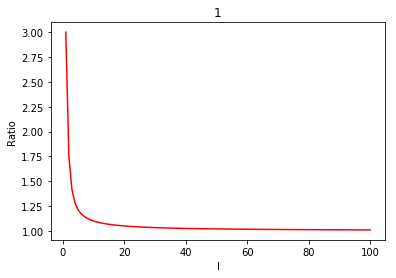
\includegraphics[width=\textwidth]{RandoK1.png}
%            \caption{$K$ set to 1}
%            \label{a}
%    \end{subfigure}
%    \begin{subfigure}[H]{0.475\textwidth}
%            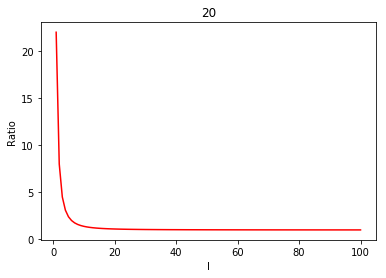
\includegraphics[width=\textwidth]{RandoK20.png}
%            \caption{$K$ set to 20}
%            \label{b}
%    \end{subfigure}
%
%    \begin{subfigure}[H]{0.475\textwidth}
%            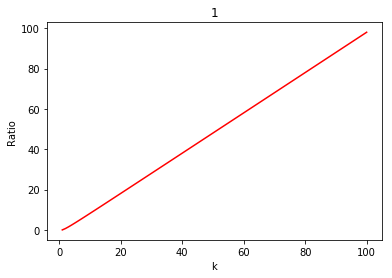
\includegraphics[width=\textwidth]{Randol1.png}
%            \caption{$L$ set to 1}
%            \label{c}
%    \end{subfigure}
%    \begin{subfigure}[H]{0.475\textwidth}
%            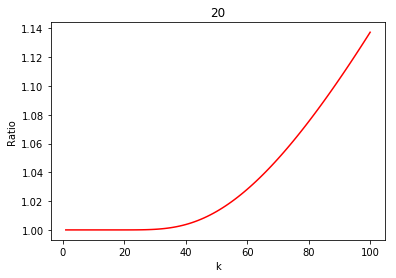
\includegraphics[width=\textwidth]{Randol20.png}
%            \caption{$L$ set to 20}
%            \label{d}
%    \end{subfigure}
%    \caption{$K$ and $L$ set to different values}\label{fig:ABCD}
%\end{figure*}
%%%


\section{Conclusion}
In this article, we have discussed the cost of distance for K-Canadian problem with deterministic approach and randomized approach, on considering different modes of communication. 

The numerical results could be useful in many applications. For example, for the cases of $T_{fd}$ and $T_{fa}$, we can judge whether a team of travelers can be more efficient in finding the target:

(1)With deterministic approach, the cost is $2K+1$ with one traveler, so it makes no difference to use multiple travelers when there is no communication($P_0$); 
\\with partial communication or complete communication, the more travelers we have, the better result we will get. Because the formula of the cost is $2(K+1)-L$ which concerns about the number of travelers, so if we want this result less than $2K+1$, we should have $L>1$.

(2)With randomised approach, the cost becomes $K+1$ for only one traveler. When there is no communication, it is complicated and we can compare the formular with $K+1$ by figures;
\\with complete communication, if we want the result better than $K+1$ which is the case of one traveler, we should have the following condition:
\[
(K+1)-(K+2-L+\frac{L(L-1)}{2(K+1)})>0
\]
so when $L>1$ and $2K+2>L$, multiple travelers can be better than only one traveler.

For future work, we recommend to explore the possibility of establishing a bi-criteria that would include both distance and time. This would expand the direct applications of the K-Canadian travelers problem for a fleet of vehicles that wants to reach destination quickly without spending to much on gas. 
Moreover, we recommend to apply the different communication systems (especially P0 et P1) with a time criteria. This would complete the previous work done by Zhang ~\cite{ZhXuQi11}.

\bibliographystyle{plain}
\bibliography{ctp.bib}

\end{document}


